% ============================================================================
% CHAPTER 2 --- PRNet: PAPR REDUCTION VIA DEEP AUTOENCODER
% ============================================================================
\chapter{PRNet: PAPR Reduction via Deep Autoencoder}
\label{ch:prnet}

The fundamental limitations of the classical PAPR reduction approaches identified in Chapter~\ref{ch:ofdm_papr} motivate a paradigm shift in transceiver design. Rather than relying on rigid algorithmic searches or intentional signal distortion, Kim et al.~\cite{kim2017novel} proposed the \textbf{PAPR Reduction Network (PRNet)}, the first deep learning-based system for joint PAPR and BER optimization in OFDM. PRNet treats the transmitter--channel--receiver chain as a single deep autoencoder: the encoder learns a data-dependent constellation mapping that jointly minimises reconstruction error and PAPR, while the decoder learns the corresponding inverse mapping, fundamentally bypassing the computational and signaling bottlenecks of classical methods.

% ============================================================================
\section{Autoencoder Framework}
\label{sec:autoencoder_framework}
% ============================================================================

In a traditional communication system, the transmitter transforms raw data into a physical signal through a rigid sequence of fixed mathematical operations, which the receiver attempts to run in reverse after the signal is distorted by the wireless channel. This physical reality maps perfectly onto the architecture of a deep learning \textbf{autoencoder}~\cite{kim2017novel}. In this framework, the neural network's \emph{encoder} acts as the transmitter, the \emph{decoder} acts as the receiver, and the mathematical layer connecting them acts as the noisy wireless channel. By placing a mathematical simulation of the channel directly between the encoder and decoder, the entire communication chain becomes a single, unified neural network.

The profound advantage of this unified architecture is that it enables \textbf{end-to-end joint training}. Rather than optimizing the transmitter and receiver as isolated digital signal processing blocks, PRNet optimises them simultaneously. This allows the network to dynamically learn a custom, data-dependent constellation mapping at the encoder that directly minimises both the reconstruction error (BER) and the peak power (PAPR), while the decoder simultaneously learns the exact inverse mapping required to recover the data despite physical channel impairments~\cite{kim2017novel}.

To realize this, PRNet integrates two trainable Deep Neural Networks (DNNs) into the communication chain. At the transmitter, the encoder DNN is placed before the IFFT, replacing the standard constellation mapper. Instead of mapping each symbol to a fixed constellation point independently, the encoder employs a fully connected structure where every output subcarrier value is a function of the \emph{entire} input block. By processing all subcarriers jointly, the encoder detects input patterns that produce high PAPR and compensates by adjusting all subcarrier amplitudes and phases to generate low-peak waveforms~\cite{kim2017novel}.

At the receiver, the decoder DNN is placed after the FFT to replace the standard constellation de-mapper. Mirroring the transmitter, it employs a fully connected structure to process the received OFDM block jointly. Due to joint training, the decoder's weights implicitly encode the encoder's mapping. Consequently, it reconstructs the original data from the equalized frequency-domain subcarriers without explicit side information, eliminating both the bandwidth overhead and severe failure modes associated with SI errors in classical methods~\cite{kim2017novel}.

\begin{figure}[H]
    \centering
    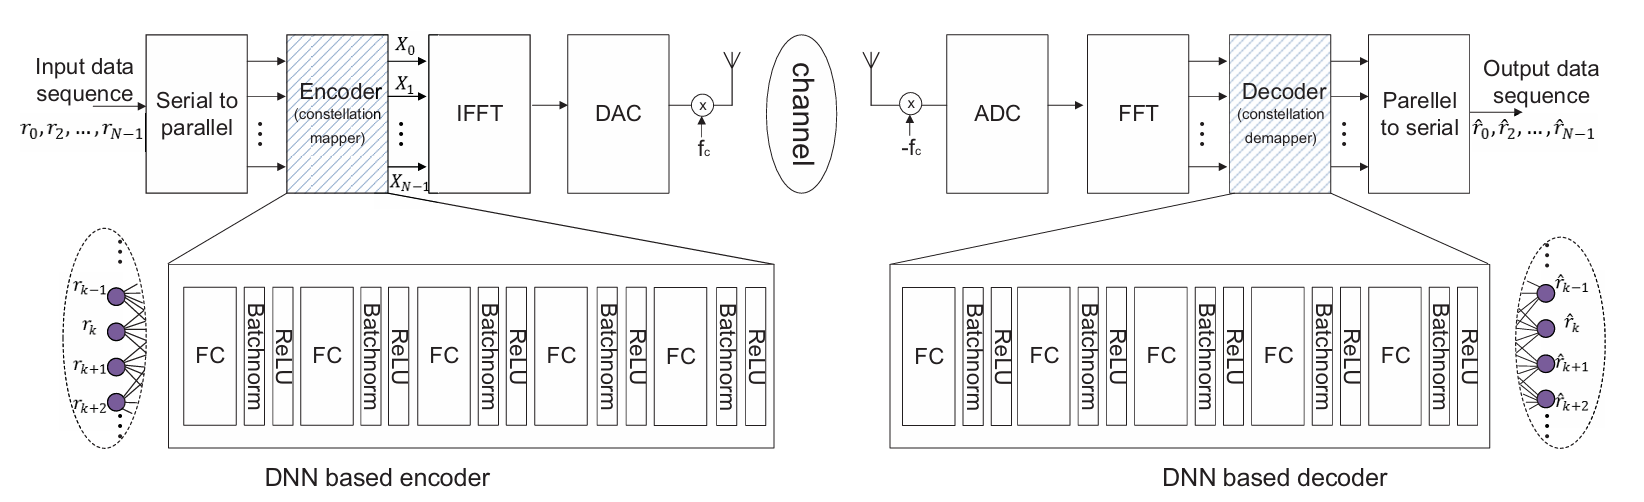
\includegraphics[width=0.95\linewidth]{Figures/PRNet/prnet_architecture.png}
    \caption{Structure of the PRNet system with DNN encoder and DNN decoder. Both consist of fully connected (FC) layers with Batch Normalization and ReLU activation. The encoder shapes the constellation before the IFFT to reduce PAPR; the decoder reconstructs the transmitted symbols after the channel and FFT~\cite{kim2017novel}.}
    \label{fig:prnet_architecture}
\end{figure}

\subsection{Core Neural Network Components}

Internally, both the encoder and decoder are constructed from identical repeated sub-blocks~\cite{kim2017novel}. Each sub-block consists of three fundamental deep learning operations applied in sequence:

\begin{itemize}
    \item \textbf{Fully Connected (FC) Layer:} Unlike standard OFDM where each subcarrier is mapped independently, the FC layers apply a linear transformation that combines the entire input vector. This dense connectivity enables the network to process all subcarriers jointly, recognising block-wide patterns that cause high PAPR and adjusting all subcarrier phases and amplitudes simultaneously.
    \item \textbf{Batch Normalization (BN):} Inserted after the linear transformations, BN standardises the intermediate constellation representations across each training batch. This stabilization is critical for PRNet, as it prevents vanishing gradients and allows the network to converge on a highly complex, multidimensional constellation mapping without training collapse.
    \item \textbf{ReLU Activation:} The Rectified Linear Unit provides the essential nonlinearity. Without it, the entire multi-layer network would collapse into a single linear matrix projection, which is mathematically insufficient to discover the highly non-convex mappings required to jointly minimize PAPR and BER.
\end{itemize}

% ============================================================================
\section{System Model}
\label{sec:system_model}
% ============================================================================

With the core neural network components established, we now formulate the PRNet transceiver as an end-to-end OFDM communication system~\cite{kim2017novel}. The system is mathematically defined for $N$ orthogonal subcarriers and an input sequence of $M$-bit symbols. For training and evaluation, we adopt the baseline configuration from Kim et al.~\cite{kim2017novel}, specifically $N = 64$ subcarriers and QPSK modulation ($M = 2$).

\subsection{Input Representation}

The original PRNet formulation~\cite{kim2017novel} maps input sequences using $256$-dimensional one-hot encoded vectors. This work replaces this categorical approach with a continuous real-valued in-phase and quadrature (I/Q) representation. Because standard deep neural networks operate exclusively in the real domain, they cannot process complex-valued OFDM symbols natively. To construct the necessary real-valued input, the $64$ complex data symbols (each representing $2$ bits) are explicitly decomposed into their in-phase ($I$) and quadrature ($Q$) components. The input sequence is thus defined as the $128$-dimensional real-valued vector:
\begin{equation*}
    \bm{r} = [I_0,\, Q_0,\, I_1,\, Q_1,\, \dots,\, I_{N-1},\, Q_{N-1}]^T \in \mathbb{R}^{2N}.
\end{equation*}

While mathematically equivalent to the one-hot formulation in achieving optimal BER and PAPR, the continuous I/Q parameterization is adopted to provide three strict architectural advantages. First, it reduces the input dimension from $256$ to $128$, strictly halving the parameter complexity of the initial projection matrix. Second, bypassing categorical encoding eliminates discrete mapping layers, allowing the network to optimize continuous physical coordinate geometry directly. Finally, it enables explicit per-symbol power normalization during the forward pass. This guarantees the strict physical constraint $\mathbb{E}[|X|^2] = 1$ for every individual transmitted waveform, overcoming the reliance on global batch-wide statistical approximations.

\subsection{DNN Encoder}

The transmitter is parameterized by the deep neural network $f(\cdot; \theta_f)$, where $\theta_f$ denotes the complete set of trainable weights and biases. The encoder follows a topology of $L_f = 5$ consecutive hidden layers, each with a width of 2048 nodes~\cite{kim2017novel}. Crucially, its final output layer is a pure linear projection with no non-linear activation or batch normalization~\cite{kim2017novel}. This is physically necessary because the network must map symbols to unconstrained coordinates on the complex I/Q plane, which inherently requires the ability to output unbounded negative and positive spatial values.

The encoder maps the real-valued input vector $\bm{r}$ directly to a frequency-domain vector representing the generated complex constellation points:
\begin{equation*}
    \bm{X} = f(\bm{r};\,\theta_f) = \left[X_0,\, X_1,\, \dots,\, X_{N-1}\right]^T \in \mathbb{C}^N.
\end{equation*}

\subsection{OFDM Modulation}

The generated frequency-domain symbols $X_k$ are modulated onto the $N = 64$ orthogonal subcarriers via an Inverse Fast Fourier Transform (IFFT) to produce the discrete time-domain sequence $x[n]$.

The Peak-to-Average Power Ratio (PAPR) of this time-domain sequence is mathematically defined as the ratio of its maximum instantaneous power to its average power:
\begin{equation*}
    \mathrm{PAPR}\{x[n]\} = \frac{\displaystyle\max_{0 \le n \le N-1} |x[n]|^2}{\mathbb{E}[|x[n]|^2]}.
\end{equation*}

Since standard Nyquist-rate sampling ($L=1$) often fails to capture the true continuous-time peaks, accurate evaluation requires an oversampling factor of $L \ge 4$. In practice, this is executed by zero-padding the frequency-domain vector $\bm{X}$ to length $NL$ before computing the IFFT. This step ensures the discrete digital PAPR reliably bounds the maximum power of the physical analog waveform.

\subsection{Channel Model}

Following the IFFT operation, the time-domain signal is transmitted through a wireless channel before arriving at the receiver. As in the original PRNet formulation~\cite{kim2017novel}, the physical transmission is abstracted using a holistic operator $\mathbb{H}$ that models the combined effects of multipath fading and thermal noise.

\subsection{OFDM Demodulation and Equalization}

At the receiver, OFDM demodulation is executed by applying an $N = 64$-point Fast Fourier Transform (FFT) to convert the received time-domain sequence $y[n]$ back into the frequency-domain symbols $Y_k$.

Following the FFT, the transmission is modeled as a Rayleigh flat-fading environment. Under this model, the received signal on the $k$-th subcarrier is mathematically defined as $Y_k = H_k X_k + E_k$, where $H_k$ represents the complex channel fading coefficient and $E_k$ represents the additive white Gaussian noise (AWGN).

To compensate for the fading effects prior to neural network decoding, Zero-Forcing (ZF) equalization is applied. Assuming perfect Channel State Information (CSI)—meaning the receiver perfectly knows $H_k$—the equalized symbols are obtained by dividing the received signal by the channel coefficient:
\begin{equation*}
    \hat{Y}_k = \frac{Y_k}{H_k} = X_k + \frac{E_k}{H_k}.
\end{equation*}

\subsection{DNN Decoder}

The receiver is parameterized by the deep neural network $g(\cdot; \theta_g)$, where $\theta_g$ denotes the complete set of trainable weights and biases. The decoder shares a symmetric topology with the encoder, comprising $L_g = 5$ consecutive hidden layers, each with a width of 2048 nodes~\cite{kim2017novel}. Similarly, its final output layer is a pure linear projection with no non-linear activation. This is required to allow the network to reconstruct unconstrained I/Q coordinate values from the noisy equalized signal prior to hard-decision demodulation.

The decoder maps the equalized frequency-domain vector $\hat{\bm{Y}}$ back to the $128$-dimensional real-valued reconstructed sequence $\hat{\bm{r}}$. A hard-decision demodulator is subsequently applied to $\hat{\bm{r}}$ to recover the original transmitted bits.

Consequently, the complete end-to-end reconstructed symbol vector at the receiver can be written as a composite function of the entire transceiver pipeline:
\begin{equation*}
    \hat{\bm{r}} = g \circ \mathrm{FFT} \circ \mathbb{H} \circ \mathrm{IFFT} \circ f(\bm{r}),
\end{equation*}
where $\mathbb{H}$ abstractly denotes the physical effects of the wireless channel. Since every block in this composite chain is mathematically differentiable, gradients from the training loss function flow backward through the entire system during joint optimization of the encoder and decoder parameters.

% ============================================================================
\section{Training Methodology}
\label{sec:training}
% ============================================================================

\subsection{Loss Function}

PRNet optimises two competing objectives simultaneously: reconstruction accuracy (low BER) and peak suppression (low PAPR). While the original PRNet formulation utilizes Cross-Entropy loss for its categorical one-hot encoded inputs~\cite{kim2017novel}, our continuous I/Q parameterization requires a regression-based loss. Thus, the reconstruction loss is formulated as the Mean Squared Error (MSE) between the original continuous input vector and the reconstructed output vector in the $2N$-dimensional real space:
\begin{equation*}
    \mathcal{L}_1(\bm{r},\hat{\bm{r}})
    = \frac{1}{2N}\bigl\|\bm{r} - g\bigl(\mathrm{FFT}(\mathbb{H} \circ \mathrm{IFFT}(f(\bm{r}; \theta_f)) + \epsilon); \theta_g\bigr)\bigr\|_2^2
    = \frac{1}{2N}\sum_{i=0}^{2N-1}\bigl(r_i - \hat{r}_i\bigr)^2.
\end{equation*}

The PAPR penalty directly measures the peak-to-average power ratio of the time-domain waveform $x[n]$~\cite{kim2017novel}. To explain how this penalty actually trains the neural network, we mathematically trace $x[n]$ back to its source: the encoder. By expanding $x[n]$ into $\mathrm{IFFT}\bigl(f(\bm{r}; \theta_f)\bigr)$, the formula explicitly shows how the PAPR loss backpropagates through the IFFT block to optimize the encoder's internal weights $\theta_f$:
\begin{equation*}
    \mathcal{L}_2(\bm{r})
    = \mathrm{PAPR}\bigl\{\mathrm{IFFT}\bigl(f(\bm{r}; \theta_f)\bigr)\bigr\}
    = \frac{\displaystyle\max_{0 \le n \le NL-1} |x[n]|^2}
    {\displaystyle\frac{1}{NL}\sum_{n=0}^{NL-1}|x[n]|^2}.
\end{equation*}

Finally, the complete joint loss function is a weighted combination of both the reconstruction loss and the PAPR penalty~\cite{kim2017novel}:
\begin{equation*}
    \mathcal{L}(\bm{r},\hat{\bm{r}})
    = \mathcal{L}_1(\bm{r},\hat{\bm{r}}) + \lambda\,\mathcal{L}_2(\bm{r}),
\end{equation*}
where $\lambda > 0$ is a weighting hyperparameter that governs the fundamental physical trade-off between reconstruction accuracy and PAPR reduction. A higher $\lambda$ forces the network to aggressively reduce PAPR, but doing so requires distorting the transmitted constellation. This distortion shrinks the minimum distance between adjacent constellation points, which inherently degrades the decoder's ability to safely recover symbols under noise, leading to a higher BER. Therefore, the chosen value of $\lambda$ dictates the balance of this trade-off.

\subsection{Two-Stage Training Procedure}

To force the decoder to learn robust decision boundaries, Kim et al.\ employ denoising autoencoder training, where artificial noise at a corruption level $\eta$ (the noise-to-signal ratio) is injected during the forward pass (the simulated transmission of the signal through the physical channel before reaching the decoder)~\cite{kim2017novel}:
\begin{equation*}
    \eta = \frac{\mathbb{E}\bigl[|\epsilon|^2\bigr]}
    {\mathbb{E}\bigl[|\bm{r}|^2\bigr]}.
\end{equation*}

Selecting $\eta$ poses a critical trade-off: insufficient noise yields overly tight decision boundaries that fail in real channels, while excessive noise prevents distinguishing adjacent constellation points. To resolve this and evaluate optimal parameters, Kim et al.\ established a two-stage training procedure~\cite{kim2017novel}:

\begin{enumerate}
    \item \textbf{Stage~1 --- Corruption level selection:} Multiple models are trained using solely the reconstruction loss $\mathcal{L}_1$ (setting $\lambda = 0$) across a sweeping range of $\eta$ values. The models are evaluated across a full SNR sweep to empirically determine the optimal noise injection level $\eta^\star$, as shown below.

          \begin{figure}[H]
              \centering
              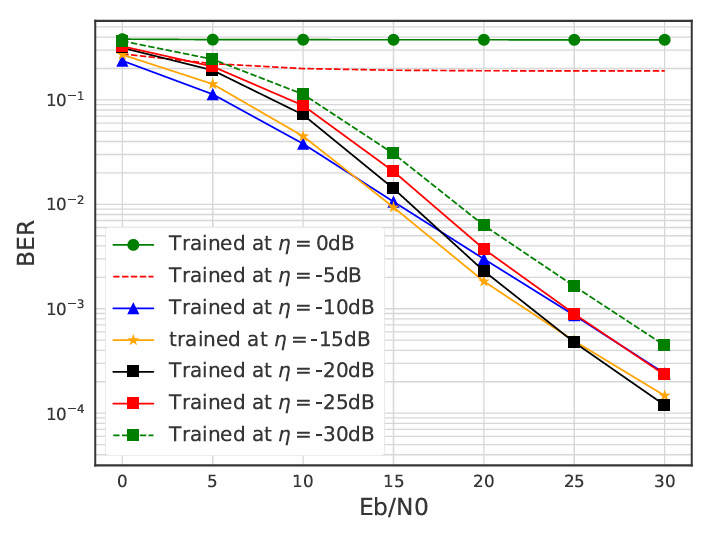
\includegraphics[width=0.55\linewidth]{Figures/PRNet/prnet_ber_corruption.png}
              \caption{BER of PRNet trained at different corruption levels $\eta$. The model trained at $\eta = -15$~dB consistently yields the lowest BER~\cite{kim2017novel}.}
              \label{fig:prnet_ber_corruption}
          \end{figure}

          The authors' results physically validate the noise trade-off: models trained at excessive corruption levels (e.g., $\eta = 0$~dB and $\eta = -5$~dB) fail to learn meaningful boundaries entirely, resulting in flat BER curves. Conversely, models trained at very low corruption levels (e.g., $\eta = -30$~dB) overfit to the noiseless scenario, yielding sub-optimal BER performance under real channel conditions. As the corruption level diverges in either direction from the optimal point, the overall BER steadily increases. Based on these empirical findings, Kim et al.\ conclude that $\eta^\star = -15$~dB strikes the perfect balance~\cite{kim2017novel}.

    \item \textbf{Stage~2 --- Joint training:} The noise injection is fixed at $\eta^\star = -15$~dB, and models are trained using the full joint loss $\mathcal{L} = \mathcal{L}_1 + \lambda\,\mathcal{L}_2$ to investigate how the penalty weight $\lambda$ dictates the trade-off between PAPR reduction and BER degradation, as illustrated below.

          \begin{figure}[H]
              \centering
              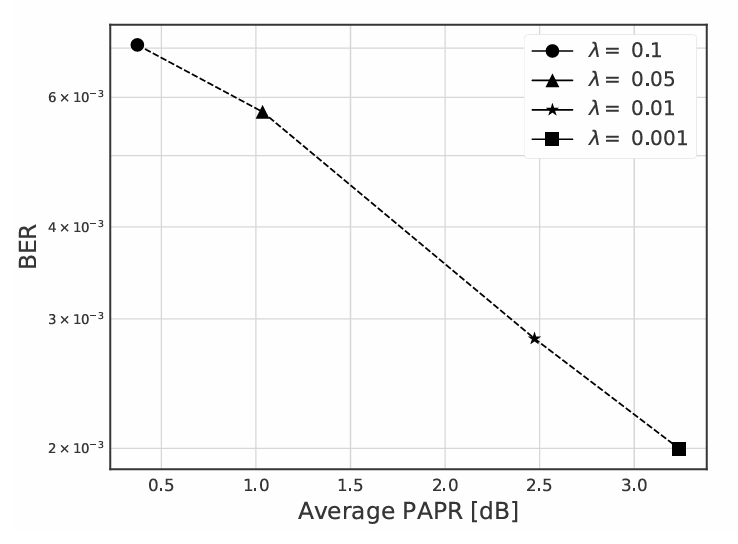
\includegraphics[width=0.55\linewidth]{Figures/PRNet/prnet_ber_papr_lambda.png}
              \caption{BER vs.\ average PAPR by varying $\lambda$ at SNR $= 20$~dB. Larger $\lambda$ reduces PAPR but increases BER~\cite{kim2017novel}.}
              \label{fig:prnet_ber_lambda}
          \end{figure}

          As established by Kim et al., as $\lambda$ increases, PAPR decreases monotonically while the BER increases, confirming the fundamental physical tension between constellation shaping and minimum distance. Heavy penalties (e.g., $\lambda = 0.1$) aggressively squash the waveform but severely compromise the error rate, whereas minimal penalties (e.g., $\lambda = 0.001$) prioritize a low BER at the expense of higher PAPR. Following this optimization sweep, the authors identified $\lambda = 0.01$ as the ideal practical operating point—striking a balance that achieves meaningful PAPR reduction without severely degrading the BER baseline~\cite{kim2017novel}.
\end{enumerate}

\newpage
% ============================================================================
\section{Simulation}
\label{sec:simulation}
% ============================================================================

\subsection{Simulation Parameters}

\begin{table}[H]
    \centering
    \caption{PRNet simulation parameters~\cite{kim2017novel}.}
    \label{tab:prnet_params}
    \begin{tabular}{@{} l l @{}}
        \toprule
        \textbf{Parameter}                      & \textbf{Value}                         \\
        \midrule
        Number of subcarriers ($N$)             & 64                                     \\
        Modulation                              & 4-QAM/QPSK                             \\
        Network input representation            & $2N=128$ real entries (I/Q components) \\
        Hidden processing blocks per DNN        & 5                                      \\
        Hidden nodes per layer                  & 2048                                   \\
        Activation function                     & ReLU (hidden), Linear (output)         \\
        Batch normalization                     & Yes, after every FC layer              \\
        Optimiser                               & Adam                                   \\
        Learning rate                           & $10^{-4}$                              \\
        Batch size                              & 400                                    \\
        Training steps                          & 500{,}000                              \\
        Optimal corruption level ($\eta^\star$) & $-15$~dB                               \\
        PAPR weight ($\lambda$)                 & 0.01                                   \\
        Evaluation size                         & 50{,}000 random OFDM sequences         \\
        \bottomrule
    \end{tabular}
\end{table}

Note that while the original paper denotes ReLU for all layers, our implementation utilizes continuous I/Q representation and MSE loss rather than one-hot classification. Therefore, a Linear activation is physically required at the final layer to allow the network outputs to span the full complex plane (both positive and negative values).

\subsection{BER Performance}

\begin{figure}[H]
    \centering
    \begin{subfigure}[b]{0.48\textwidth}
        \centering
        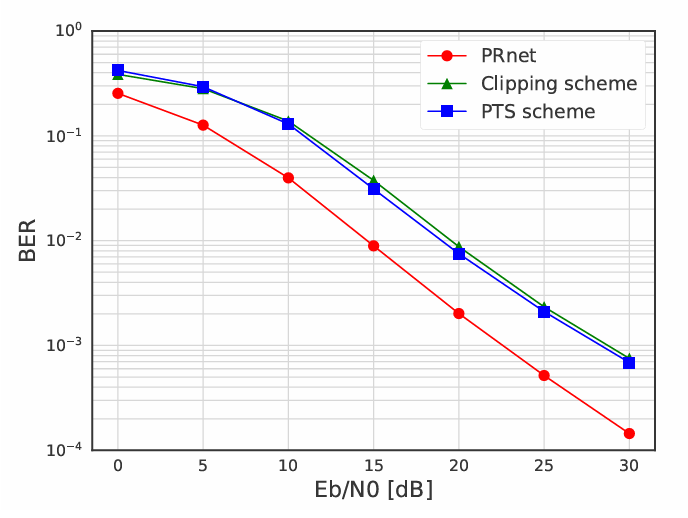
\includegraphics[width=\textwidth]{Figures/PRNet/prnet_ber.png}
        \caption{Results from the original paper~\cite{kim2017novel}}
        \label{fig:prnet_ber_paper}
    \end{subfigure}
    \hfill
    \begin{subfigure}[b]{0.48\textwidth}
        \centering
        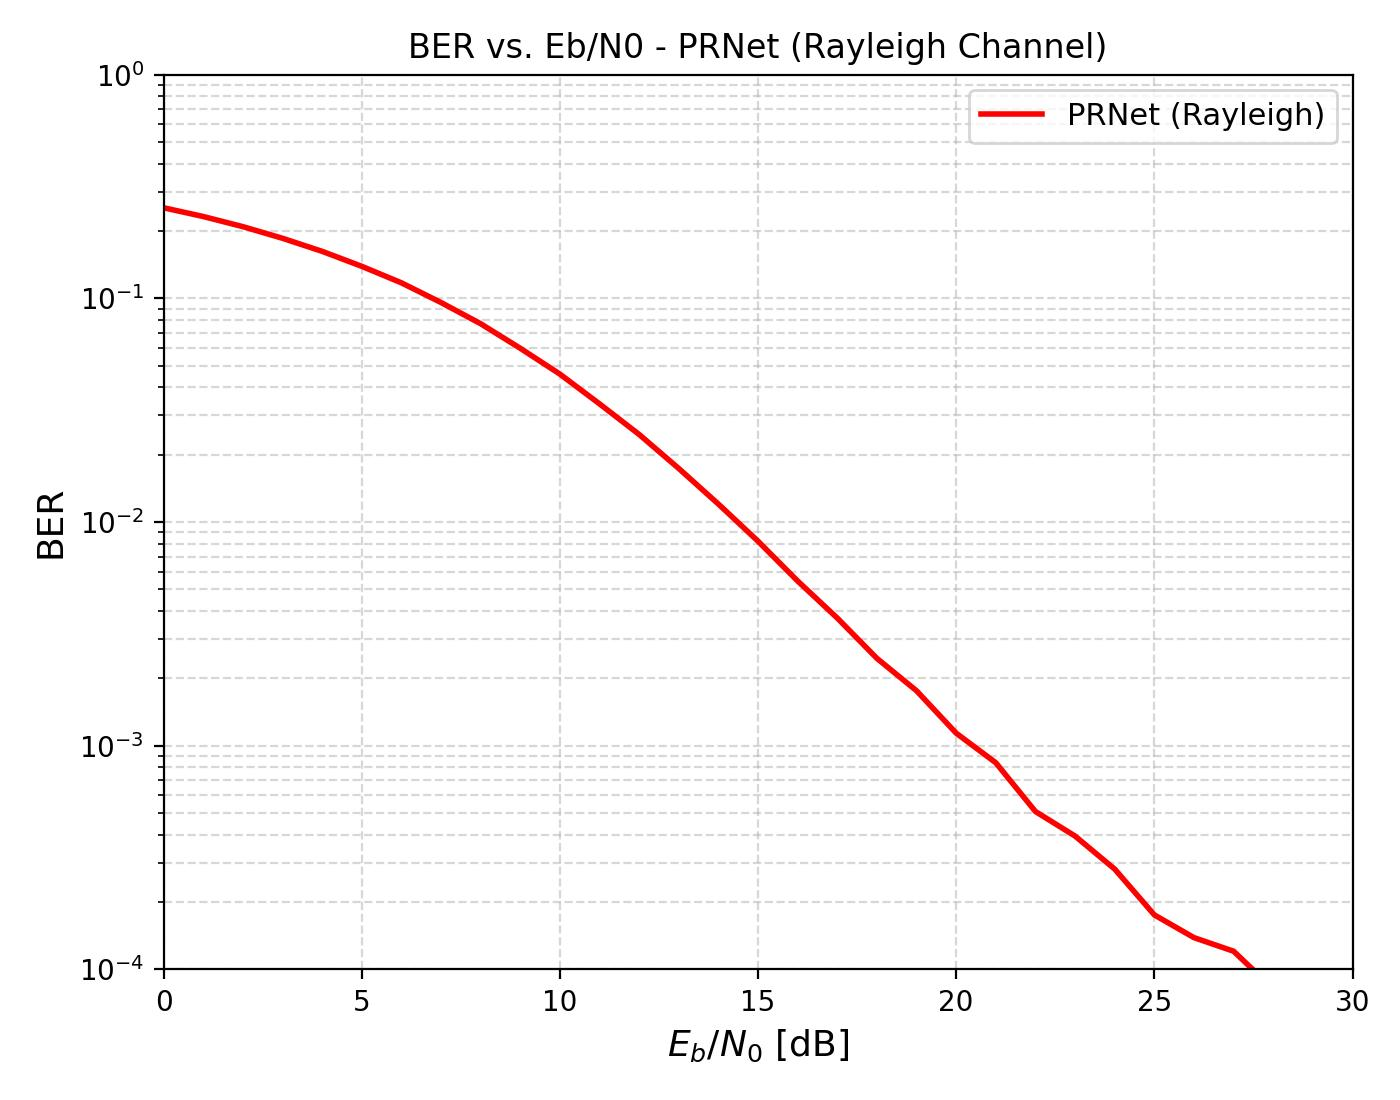
\includegraphics[width=0.96\textwidth]{Figures/PRNet/PRNet - Results/ber_vs_snr_rayleigh.jpg}
        \caption{Our simulated results}
        \label{fig:prnet_ber_reproduced}
    \end{subfigure}
    \caption{BER vs.\ SNR performance of PRNet. Both the (a) original paper and (b) our reproduction demonstrate consistent BER performance.}
    \label{fig:prnet_ber}
\end{figure}

As observed in Figure~\ref{fig:prnet_ber}, the BER performance of our reproduced model is highly consistent with the results reported by the original authors. PRNet acts as a highly efficient deterministic function requiring zero iterative searching or side information during inference, validating the robustness of the deep learning approach~\cite{kim2017novel}.

\subsection{PAPR Reduction}

The CCDF evaluation demonstrates a substantial reduction in the PAPR of the PRNet-shaped symbols. The authors report that the probability of the PAPR exceeding 3~dB is less than $10^{-3}$~\cite{kim2017novel}. However, a mathematical critique of the authors' open-source code (\url{https://github.com/gomman/OFDM_PAPR_reduction}) reveals a metric discrepancy: the CCDF is plotted using an amplitude-based proxy rather than the standard power-based definition. Specifically, their implementation computes the metric as:
\begin{equation*}
    \mathrm{PAPR}_{\mathrm{proxy}}\,\mathrm{[dB]} = 10\log_{10}\left(\max_{n} \lvert x_{\mathrm{norm}}[n] \rvert\right),
\end{equation*}
where $x_{\mathrm{norm}}[n]$ represents the time-domain symbol normalized to unit average power. In contrast, the standard physical PAPR (in dB) is a true power ratio, defined mathematically as:
\begin{equation*}
    \mathrm{PAPR}_{\mathrm{standard}}\,\mathrm{[dB]} = 10\log_{10}\left(\max_{n} \lvert x_{\mathrm{norm}}[n] \rvert^2\right) = 20\log_{10}\left(\max_{n} \lvert x_{\mathrm{norm}}[n] \rvert\right).
\end{equation*}
Consequently, the proxy metric is mathematically exactly half of the standard physical PAPR in decibels ($\mathrm{PAPR}_{\mathrm{standard}}\,\mathrm{[dB]} = 2\cdot \mathrm{PAPR}_{\mathrm{proxy}}\,\mathrm{[dB]}$).

As shown in Figure~\ref{fig:prnet_ccdf}, evaluating the model using the authors' proxy metric perfectly reproduces the 3~dB curve reported in the original paper, confirming the consistency of our reproduced architecture. However, evaluating the trained model under the standard physical metric yields a realistic PAPR of approximately 6~dB at a CCDF of $10^{-3}$. This still represents a substantial 4--5~dB reduction from the original OFDM baseline (typically 10--11~dB), validating PRNet's exceptional PAPR reduction capabilities despite the metric discrepancy.

\begin{figure}[H]
    \centering
    \begin{subfigure}[b]{0.48\textwidth}
        \centering
        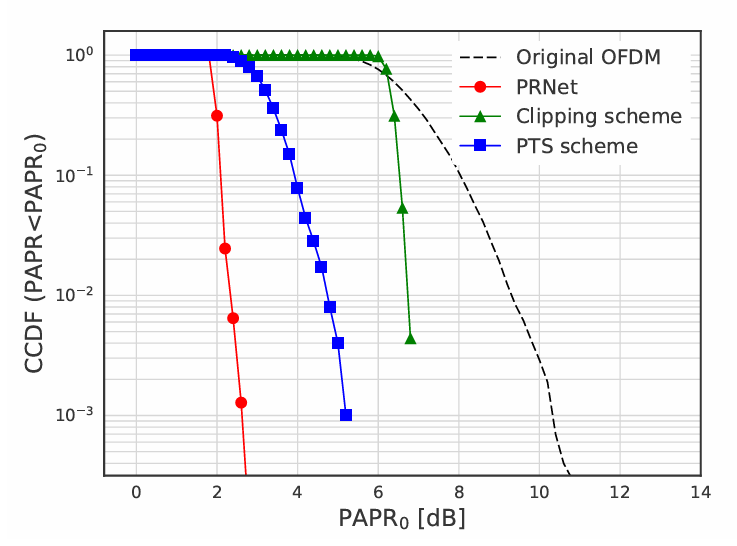
\includegraphics[width=\textwidth]{Figures/PRNet/prnet_ccdf.png}
        \caption{Results from the original paper~\cite{kim2017novel}}
        \label{fig:prnet_ccdf_paper}
    \end{subfigure}
    \hfill
    \begin{subfigure}[b]{0.48\textwidth}
        \centering
        
\includegraphics[width=0.94\textwidth]{Figures/PRNet/PRNet - Results/ccdf_papr_rayleigh.jpg}
        \caption{Our simulated results}
        \label{fig:prnet_ccdf_reproduced}
    \end{subfigure}
    \caption{CCDF of PAPR performance for PRNet. Both the (a) original paper and (b) our reproduction demonstrate a consistent 3~dB curve when using the authors' proxy metric. However, our reproduction validates that the standard physical metric yields a realistic 6~dB PAPR, which still significantly outperforms the original OFDM baseline.}
    \label{fig:prnet_ccdf}
\end{figure}

\subsection{Learned Constellation Shaping}

To understand how PRNet achieves this implicit coding gain while simultaneously reducing PAPR, it is instructive to examine the raw output of the encoder. Unlike classical OFDM, which enforces rigidly discrete QPSK boundaries, the PRNet encoder learns to dynamically distort and disperse the constellation points.

Figure~\ref{fig:prnet_constellation} visualizes the complex output symbols generated by the trained encoder. By mapping the discrete input data into this continuous, cloud-like spatial distribution, the network successfully trades off traditional Euclidean spacing to achieve optimal PAPR reduction and joint source-channel coding over the Rayleigh fading channel.

\begin{figure}[H]
    \centering
    
\includegraphics[width=0.45\textwidth]{Figures/PRNet/PRNet - Results/encoder_constellation_rayleigh.jpg}
    \caption{The learned constellation output of the PRNet encoder. The network disperses the traditional QPSK boundaries into a continuous distribution to minimize PAPR while preserving decodability.}
    \label{fig:prnet_constellation}
\end{figure}

\subsection{Computational Complexity}

At inference time, PRNet eliminates the need for iterative searching (like in PTS) and replaces it with a single neural network forward pass.

The original authors reported the computational complexity of this forward pass as $\mathcal{O}(L \cdot K \cdot M)$, where $L$ is the number of fully connected processing layers (5), $K$ is the hidden layer size (2048), and $M$ is the modulation order (4 for QPSK)~\cite{kim2017novel}. However, this formulation contains a mathematical error. In a fully connected network, passing data from one hidden layer to the next requires multiplying a vector of size $K$ by a weight matrix of size $K \times K$. Because $K$ is very large (2048), these hidden layer computations completely dominate the processing time. Therefore, the true theoretical complexity is $\mathcal{O}(L \cdot K^2)$, which is entirely independent of the modulation order $M$.

Despite this error in their theoretical formulation, the practical benefit remains clear: the computational cost of PRNet is fixed, meaning it does not scale exponentially with the search space like classical scrambling methods do.

\begin{table}[H]
    \centering
    \caption{Execution time comparison for different PAPR reduction methods, as reported by the original authors~\cite{kim2017novel}.}
    \label{tab:prnet_timing}
    \begin{tabular}{@{} l r @{}}
        \toprule
        \textbf{Method}             & \textbf{Execution time ($\mu$s)} \\
        \midrule
        PTS                         & 2{,}890                          \\
        Clipping and filtering      & 1{,}415                          \\
        PRNet (without parallelism) & 2{,}304                          \\
        PRNet (with GPU)            & 480                              \\
        \bottomrule
    \end{tabular}
\end{table}

As shown in Table~\ref{tab:prnet_timing}, applying GPU acceleration allows PRNet to run approximately 6 times faster than PTS and 3 times faster than clipping and filtering, all while delivering superior BER and PAPR performance~\cite{kim2017novel}.

% ============================================================================
\section{Limitations}
\label{sec:limitations}
% ============================================================================

Despite its contributions, PRNet presents several limitations that define the research agenda for subsequent work:
\begin{itemize}
    \item \textbf{Scalability Constraints:} Fully connected layers scale quadratically with the subcarrier count ($N$). While manageable for experimental $N=64$ setups, scaling to commercial $N=1024$ standards triggers a parameter explosion and prohibitive memory overhead, restricting deployment in large-scale systems.
    \item \textbf{Channel Mismatch Vulnerability:} The network severely overfits to the specific channel model used during training. Deploying PRNet in dynamic environments with unmodelled fading or imperfect channel state information degrades performance significantly.
    \item \textbf{Configuration Dependence:} The architecture relies on rigidly fixed input and output dimensions. Any real-time adjustment to the modulation order ($M$) or subcarrier count ($N$) breaks the model, requiring a full architectural redesign and retraining from scratch.
    \item \textbf{Lack of Interpretability:} The constellation shaping strategies are hidden within millions of "black-box" weights. This lack of transparency makes it mathematically impossible to provide the worst-case performance guarantees required by strict telecommunication standards.
\end{itemize}
